\section{Algorithmen}



\begin{frame}{Algorithmen für fair k-center}
    \begin{minipage}[t]{0.5\textwidth}
        \begin{itemize}
            \item vergleich 2 Verschiedener Ansätze
            \begin{itemize}
                \item Red-Clustering \footfullcite{chierichetti2018fair}
                \item Fast-Anchor-Clustering \footfullcite{BA_Clustering_Irina}
            \end{itemize}
            \item Nutzen von Fairlets
            \begin{itemize}
                \item kleinst mögliche Clustereinheit
            \end{itemize}
            \item beschränkt auf 2 Farben
            \item beide Algorithmen verallgemeinbar
            \item Aufteilung in 1:1 Cluster
        \end{itemize}
    \end{minipage}
\end{frame}















\begin{frame}{Algorithmen für fair k-center (mit Ausreißern)}
    \begin{minipage}[t]{0.5\textwidth}
        \begin{itemize}
            \item vergleich 2 Verschiedener Ansätze
            \begin{itemize}
                \item Red-Clustering \footfullcite{chierichetti2018fair}
                \item Fast-Anchor-Clustering \footfullcite{BA_Clustering_Irina}
            \end{itemize}
            \item Nutzen von Fairlets
            \begin{itemize}
                \item kleinst mögliche Clustereinheit
            \end{itemize}
            \item beschränkt auf 2 Farben
            \item beide Algorithmen verallgemeinbar
            \item Aufteilung in 1:1 Cluster
        \end{itemize}
    \end{minipage}
    \hfill
    \begin{minipage}[t]{0.45\textwidth}
        Zusatz: Ausreißer
        \begin{itemize}
            \item reelle Daten nicht perfekt 1:1
            \item so viele Ausreißer sodass 1:1
            \begin{itemize}
                \item werden nicht mehr in Cluster berücksicthigt
            \end{itemize}
            \item bei $n:n+k$ Verteilung $\rightarrow k$ Ausreißer 
        \end{itemize}
    \end{minipage} 
\end{frame}













\begin{frame}{Fairlets}
    \begin{itemize}
        \item kleinste, faire Clustereinheit
        \begin{itemize}
            \item hier 1:1 (Rot : Blau)
        \end{itemize}
        \item Nutzen von Fairlets
        \begin{itemize}
            \item Fairlets immer zusammen zu Clustern hinzufügen
            \item $\rightarrow$ Cluster immer ausgeglichen
        \end{itemize}
        \item können optimal berechnet werden über Matching
        \item Unterschied zwischen Red-Clustering und Fast-Anchor-Clustering
    \end{itemize}

\end{frame}













\begin{frame}{Red-Clustering}
    \begin{minipage}[t]{0.55\textwidth}
        \Copy{RedClusteringFluss}{
            \begin{large}
                Finden der Fairlets
            \end{large}
            \begin{itemize}
                \item bipartiter Graph mit Roten und Blauen Knoten aufbauen
                \item mit Quelle $s$ und Senke $t$ zum Flussnetzwerk machen
                \item Kanten $s \rightarrow$ Rot und Blau $\rightarrow t$ einfügen
                \item Kanten zwischen den Mengen nach Bedingung:
                \begin{itemize}
                    \item $r_{test} \geq dist(a, b)$ dann Kannte
                \end{itemize}
                \item maximaler Fluss berechnen
                \item bestes Überdeckendes Matching suchen
                \item gematchte Punkte sind Fairlets
                \item nicht gematchte Punkte $\rightarrow$ Ausreißer
            \end{itemize}
        }
    \end{minipage}
    \hfill
    \begin{minipage}[t]{0.44\textwidth}
        \vspace{-\baselineskip} % Move image to the top
        % Beispiel Flusserstellung
        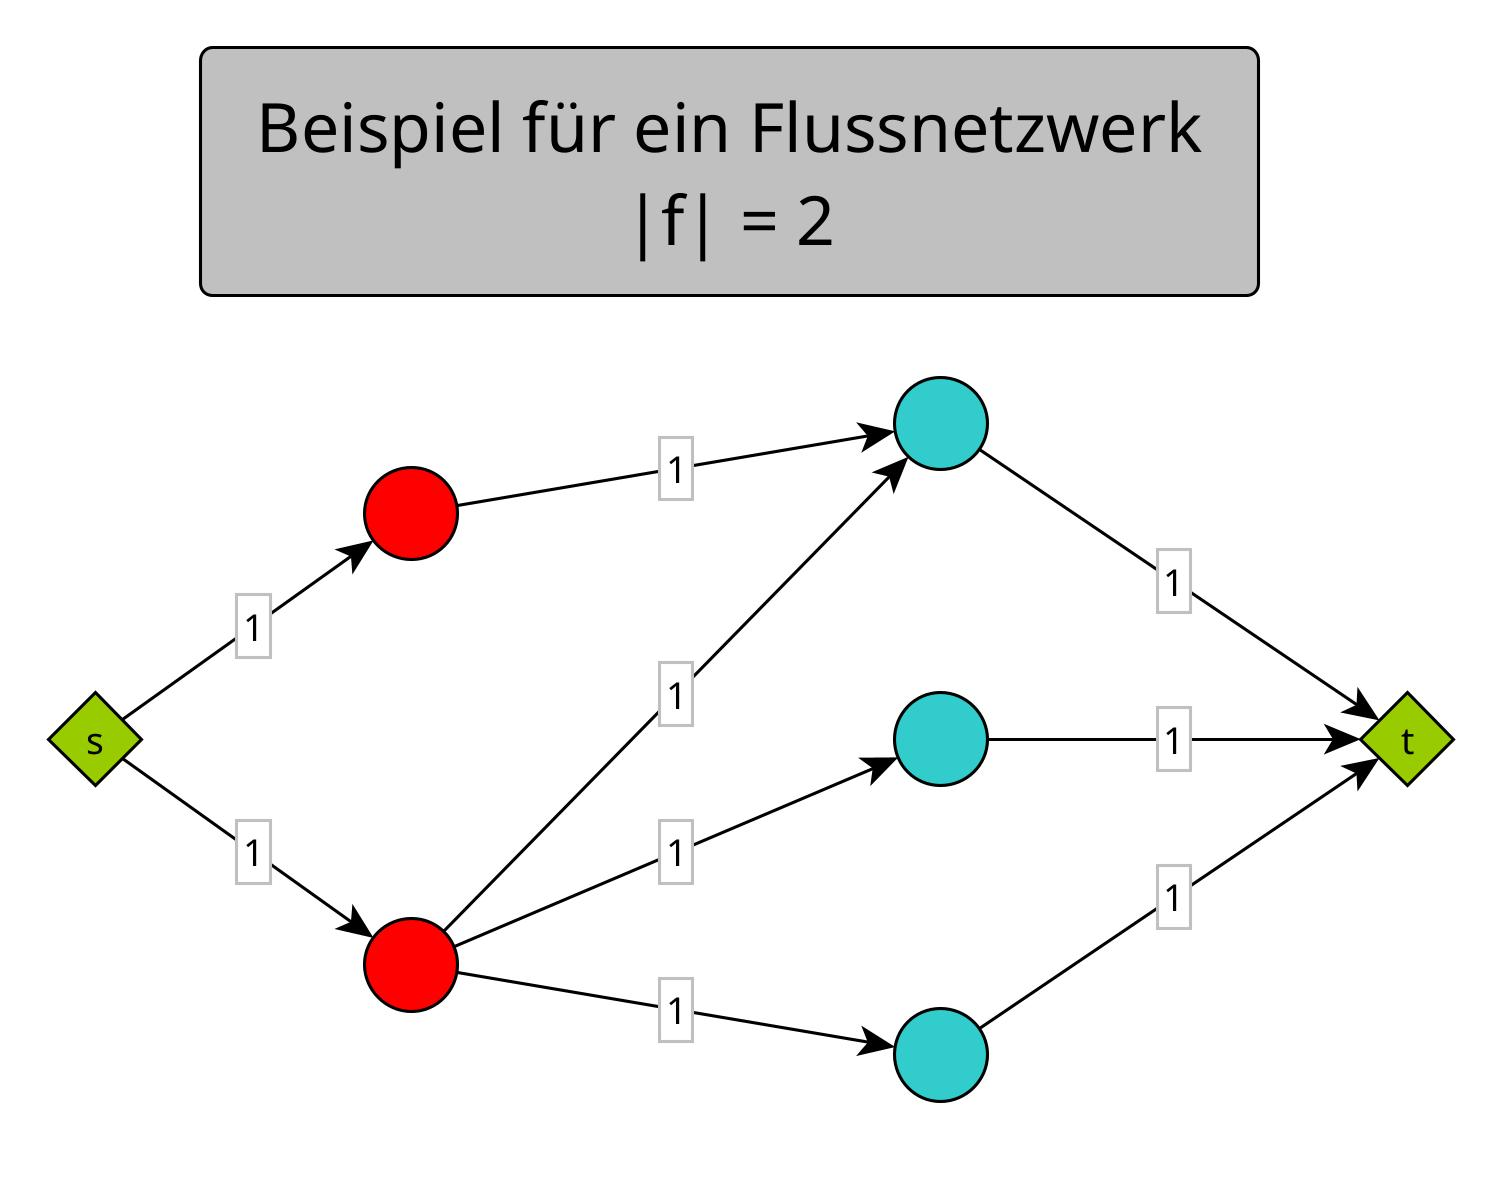
\includegraphics[width=\textwidth]{fig/Flüsse/Flussbeispiel Fairlettbildung (ohne Fluss).jpg}
    \end{minipage}
\end{frame}


\begin{frame}{Red-Clustering}
    \begin{minipage}[t]{0.55\textwidth}
        \Paste{RedClusteringFluss}
    \end{minipage}
    \hfill
    \begin{minipage}[t]{0.44\textwidth}
        \vspace{-\baselineskip} % Move image to the top
        % Beispiel Flusserstellung
        
\includegraphics[width=\textwidth]{fig/Flüsse/Flussbeispiel Fairlettbildung.jpg}
    \end{minipage}
\end{frame}















% ================= Red-Clustering Frames ================= %

\begin{frame}{Red-Clustering}
    \begin{minipage}[t]{0.40\textwidth}
        \Copy{RedClusteringAlgorithm}{
            \begin{large}
                Clustern mit Fairlets
            \end{large}
            \begin{itemize}
                \item nur Rote Punkte Clustern
                \item alle Blauen Punkte zu ihren Partnern zuweisen
            \end{itemize}
        }
    \end{minipage}
    \hfill
    \begin{minipage}[t]{0.55\textwidth}
        \vspace{-\baselineskip} % Move image to the top
        % Beispiel Fertiges Red-Clustering
        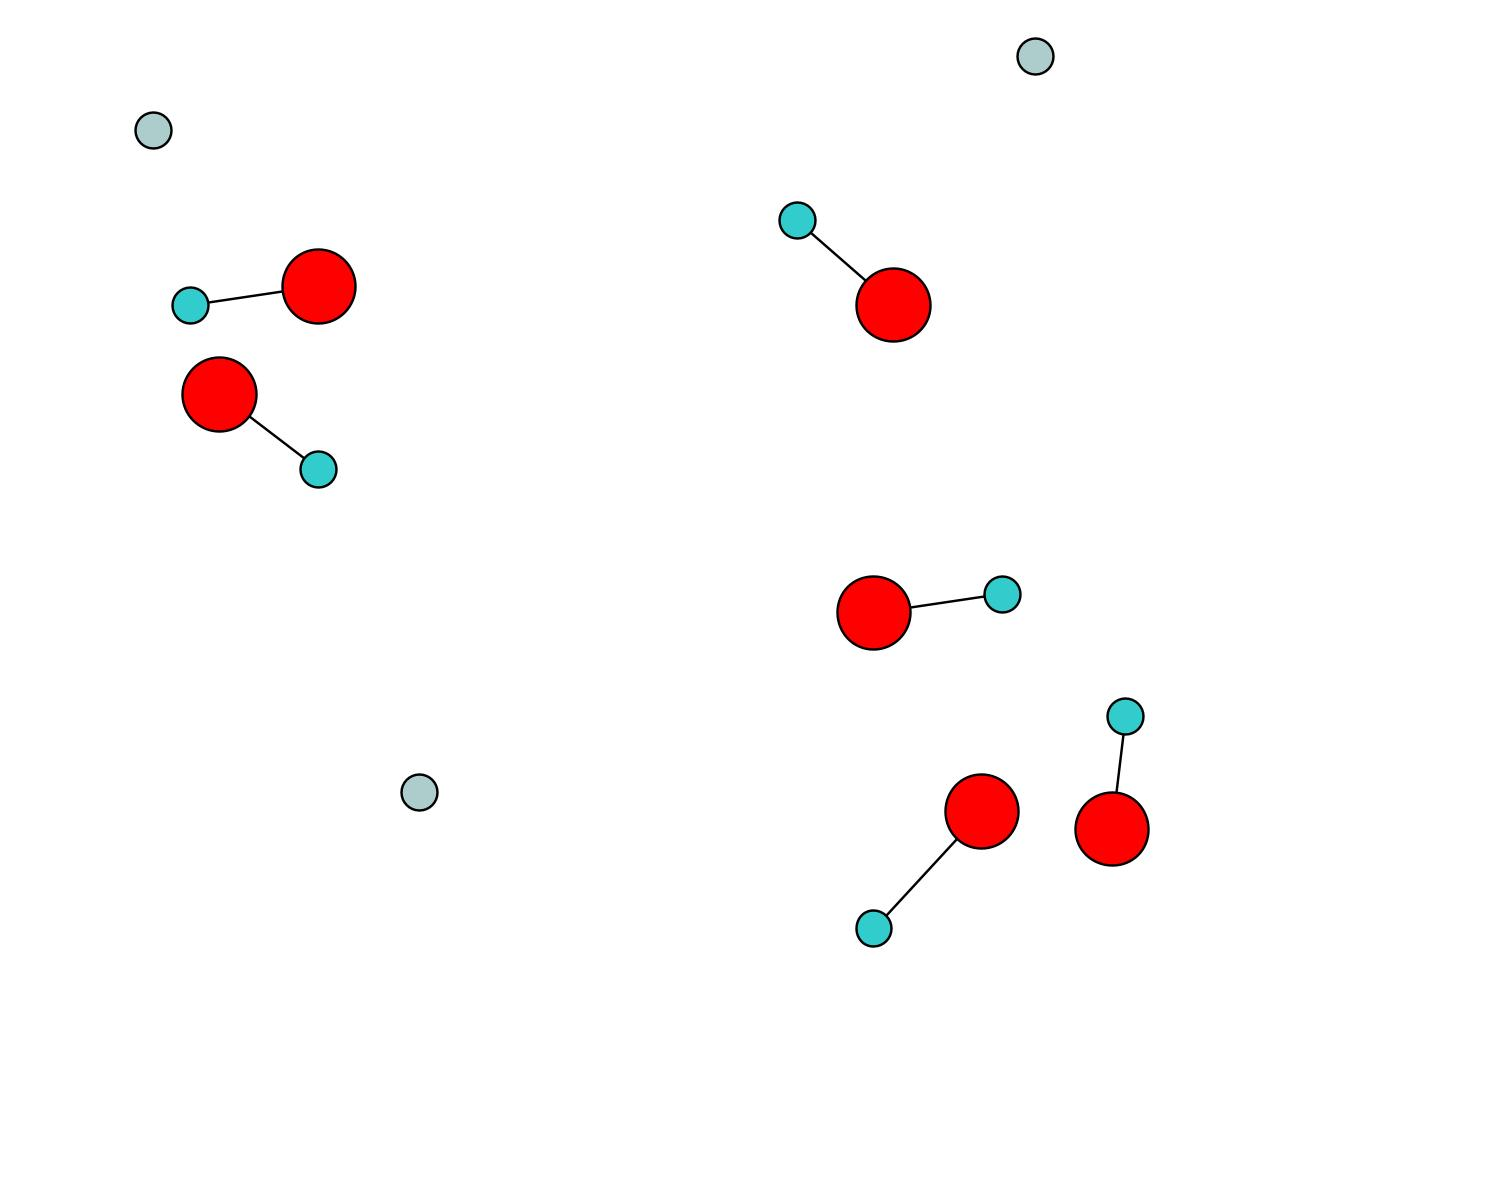
\includegraphics[width=\textwidth]{fig/Red-Clustering/Red-Clustering Ausgangslage.jpg}
    \end{minipage}
\end{frame}


\begin{frame}{Red-Clustering}
    \begin{minipage}[t]{0.40\textwidth}
        \Paste{RedClusteringAlgorithm}
    \end{minipage}
    \hfill
    \begin{minipage}[t]{0.55\textwidth}
        \vspace{-\baselineskip} % Move image to the top
        % Beispiel Fertiges Red-Clustering
        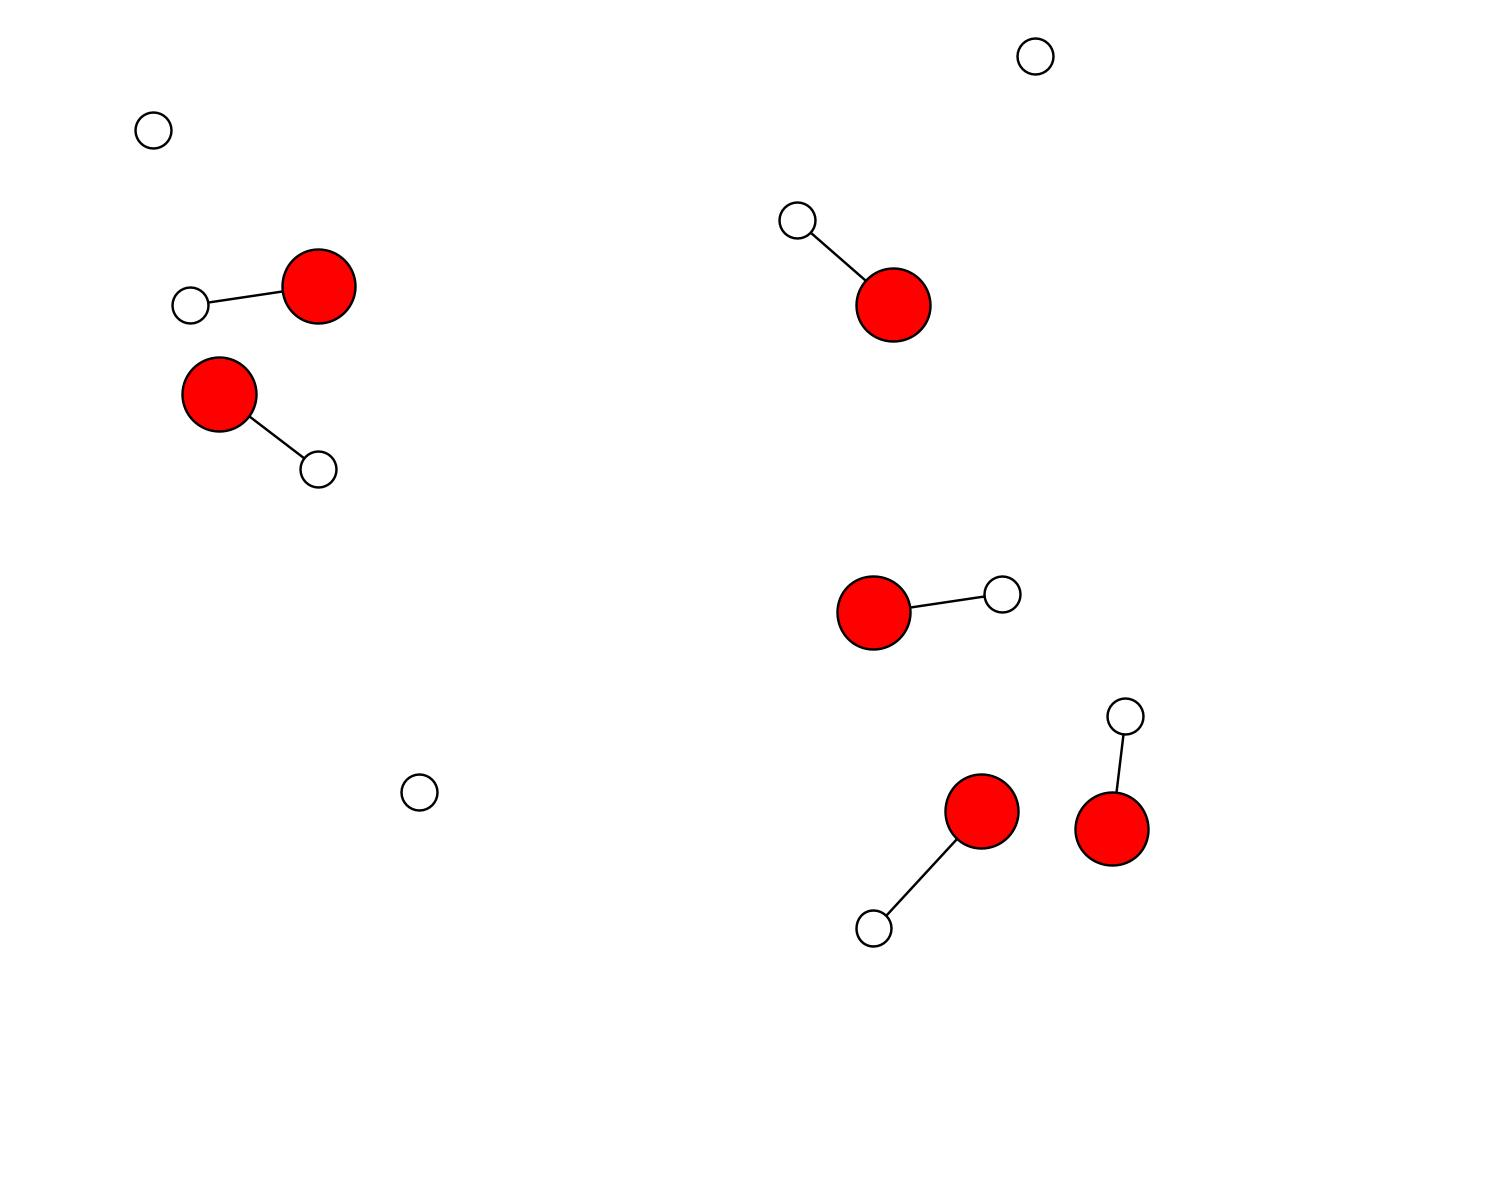
\includegraphics[width=\textwidth]{fig/Red-Clustering/Red-Clustering nur Rote.jpg}
    \end{minipage}
\end{frame}


\begin{frame}{Red-Clustering}
    \begin{minipage}[t]{0.4\textwidth}
        \Paste{RedClusteringAlgorithm}
    \end{minipage}
    \hfill
    \begin{minipage}[t]{0.55\textwidth}
        \vspace{-\baselineskip} % Move image to the top
        % Beispiel Fertiges Red-Clustering
        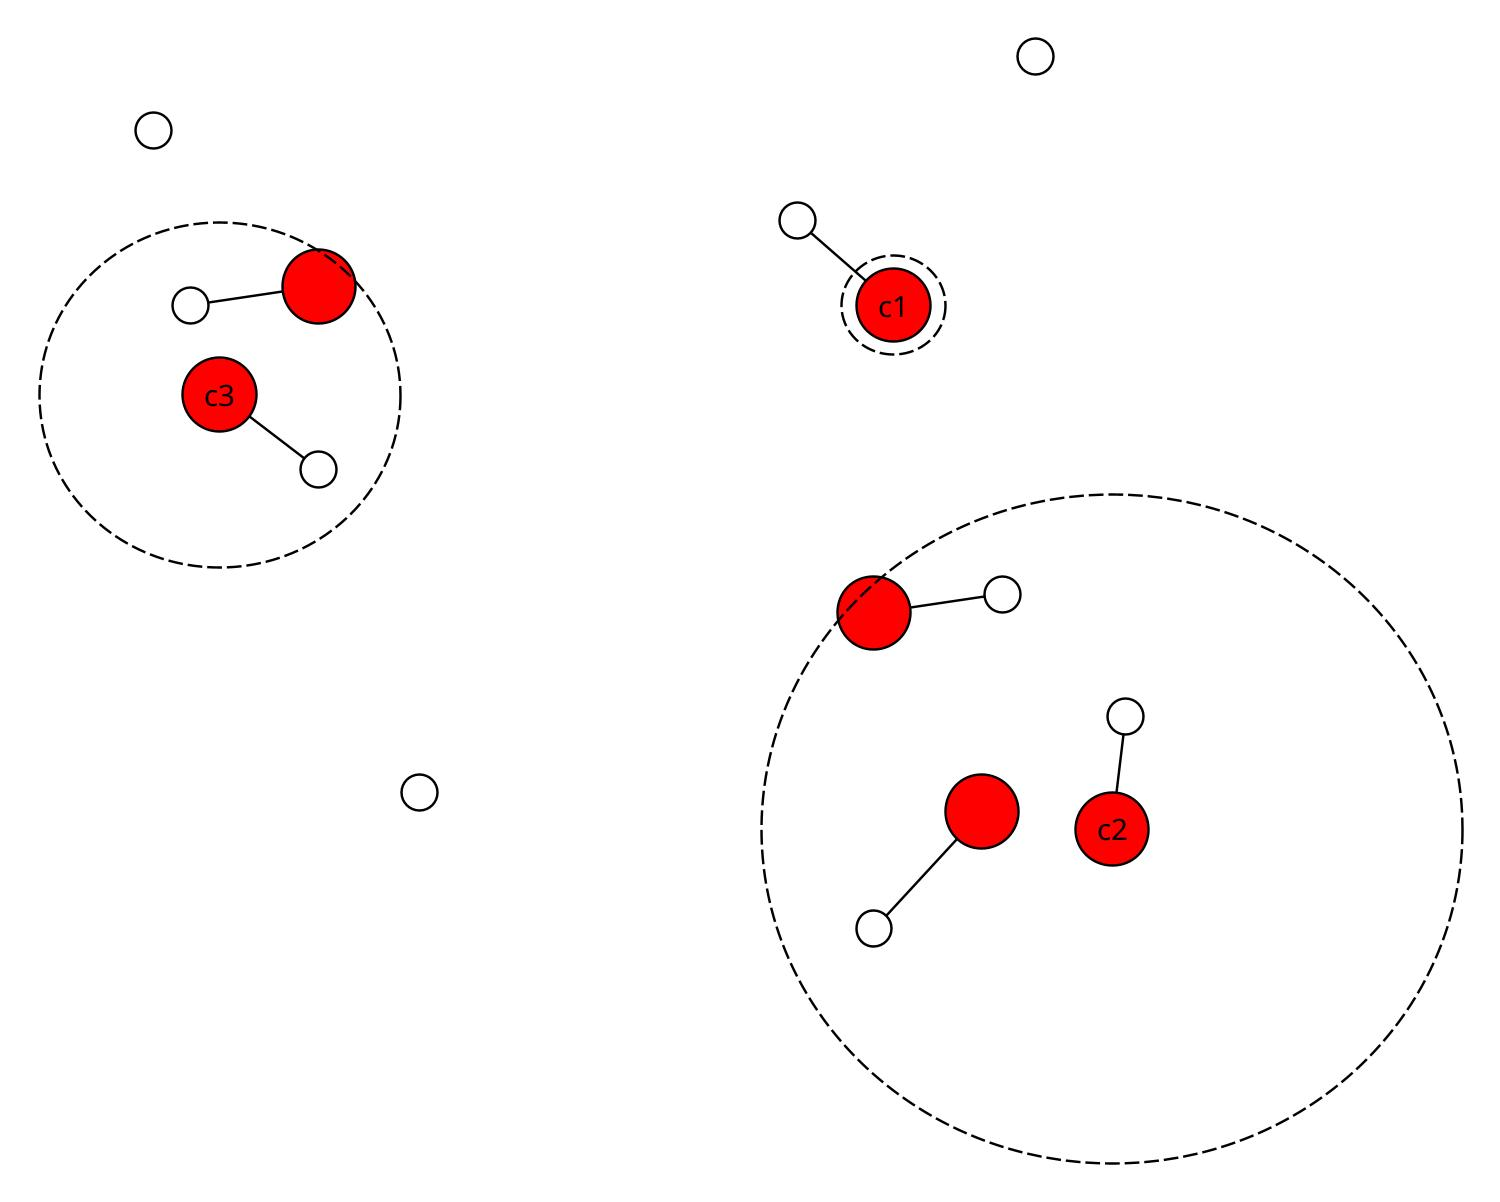
\includegraphics[width=\textwidth]{fig/Red-Clustering/Red-Clustering nach Gonzalez.jpg}
    \end{minipage}
\end{frame}


\begin{frame}{Red-Clustering}
    \begin{minipage}[t]{0.4\textwidth}
        \Paste{RedClusteringAlgorithm}
    \end{minipage}
    \hfill
    \begin{minipage}[t]{0.55\textwidth}
        \vspace{-\baselineskip} % Move image to the top
        % Beispiel Fertiges Red-Clustering
        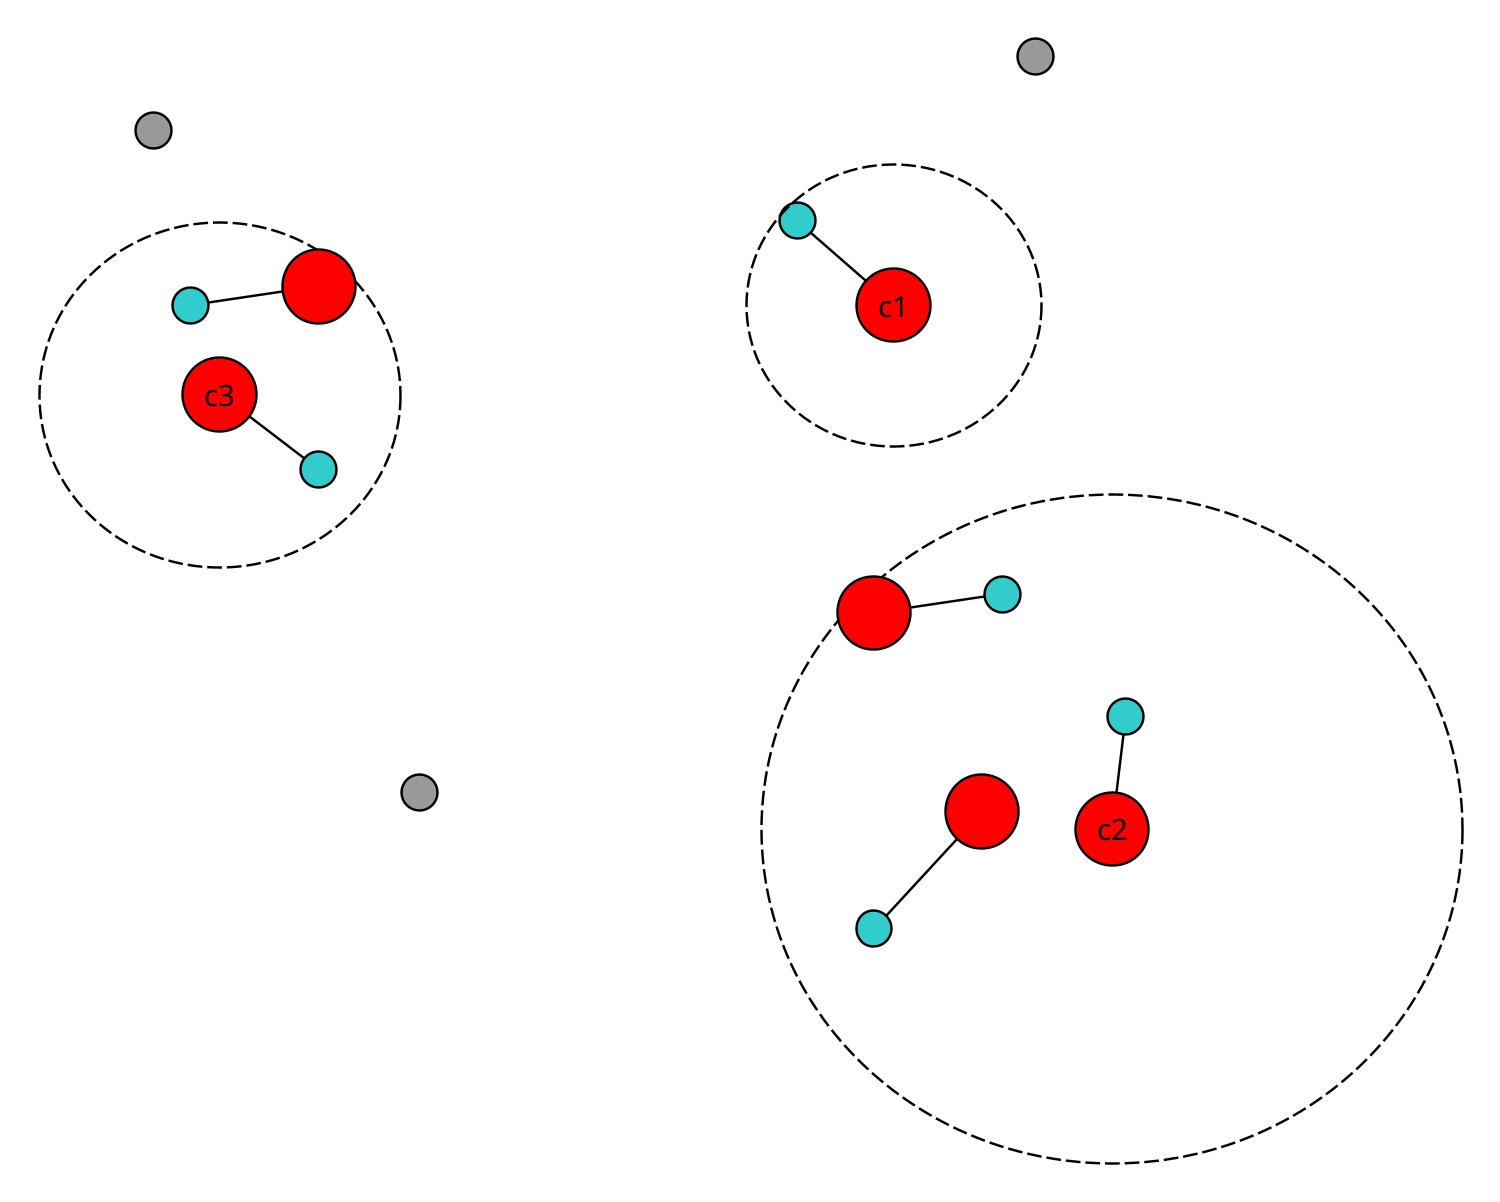
\includegraphics[width=\textwidth]{fig/Red-Clustering/Red-Clustering nach Gonzalez mit Blauzuweißung.jpg}
    \end{minipage}
\end{frame}
































\begin{frame}{Fast-Anchor-Clustering}
    \begin{minipage}[t]{0.55\textwidth}
        \begin{large}
            Finden der Fairlets - Anchor Variante
        \end{large}
        \begin{itemize}
            \item Anker für jedes Knotenpaar bestimmen
            \begin{itemize}
                \item $\rightarrow$ max Abstand der Partner zum Anker minimal
            \end{itemize}
            \begin{scriptsize}
                \item bipartiter Graph mit Roten und Blauen Knoten aufbauen
                \item mit Quelle $s$ und Senke $t$ zum Flussnetzwerk machen
                \item Kanten $s \rightarrow$ Rot und Blau $\rightarrow t$ einfügen
            \end{scriptsize}
            
            \item Kanten zwischen den Mengen nach Bedingung:
            \begin{itemize}
                \item $r_{test} \geq anchor-dist(a, b)$ dann Kannte
            \end{itemize}
            \begin{scriptsize}
                \item maximaler Fluss berechnen
                \item bestes Überdeckendes Matching suchen
                \item gematchte Punkte sind Fairlets
                \item nicht gematchte Punkte $\rightarrow$ Ausreißer
            \end{scriptsize}
            
        \end{itemize}
    \end{minipage}
    \hfill
    \begin{minipage}[t]{0.44\textwidth}
        \vspace{-\baselineskip} % Move image to the top
        % Beispiel Flusserstellung
        
\includegraphics[width=\textwidth]{fig/Flüsse/Flussbeispiel Fairlettbildung.jpg}
    \end{minipage}
\end{frame}
















\begin{frame}{Fast-Anchor-Clustering}
    \begin{minipage}[t]{0.6\textwidth}
        \begin{large}
            Clustern mit Fairlet-Anker
        \end{large}
        \begin{itemize}
            \item alle Punkte ohne Ausreißer Clustern
            \item Zentren und ihre Fairletpartner sich selbst zuweisen
            \begin{itemize}
                \item $\rightarrow$ Center-Awareness
            \end{itemize}
            \item Punkte dem nächsten Zentrum ihres Ankers zuweisen
        \end{itemize}
    \end{minipage}
    \hfill
    \begin{minipage}[t]{0.35\textwidth}
        \vspace{-\baselineskip} % Move image to the top
        % Beispiel fertiges Fast-Anchor-Clustering
        \includegraphics[width=\textwidth]{example-image-b}
    \end{minipage}
\end{frame}













\begin{frame}{Red-Clustering vs Fast-Anchor-Clustering (Theorie)}
    \begin{itemize}
        \item Red-Clustering hat Appoximationsgarantie von 4
        \item Fast-Anchor-Clustering hat Appoximationsgarantie von 3
        \item Laufzeit beider Algorithmen $\in \mathcal{O}(n^3)$
    \end{itemize}
\end{frame}

